% ===== §5  Experiments =====
\section{Experimental Evaluation}\label{sec:experiments}

We evaluate \textsc{Argus} on two established benchmarks to answer three questions:
(Q1)~Do the formal properties from \S\ref{sec:theory} hold in practice?
(Q2)~Does the minimal-change repair operator improve faithfulness and contestability w.r.t.\ existing baselines?
(Q3)~What is the empirical cost of repair?

We evaluate on 500 randomly sampled instances (seed 42) from HotpotQA~\cite{yang2018hotpotqa} (multi-hop QA) and 500 from FEVER~\cite{thorne2018fever} (fact verification).
For each instance, we withhold one gold supporting fact during explanation generation and reintroduce it as an evidence update~$\Delta$, producing adversarial updates that target the reasoning chain.
GPT-4o (\texttt{gpt-4o-2024-11-20})~\cite{openai2023gpt4} generates initial explanations (temperature 0.2); relation discovery uses DeBERTa-v3-large (MultiNLI, threshold 0.7); repairs are computed by clingo~5.6 with $k{=}3$ under uniform cost.
Results are averaged over 5 runs (std ${\leq}\,0.02$ for accuracy, ${\leq}\,0.4$ for cost).  Further details on the withholding methodology, hardware, and reproducibility are provided in Appendix~\ref{app:exp-details}.

We measure four metrics.
\emph{Faithfulness} is the fraction of argument units whose removal (counterfactual ablation) changes the answer; baselines without structured units undergo the same LLM-based decomposition before ablation (details in Appendix~\ref{app:exp-details}).
\emph{Contestability} is the fraction of gold counterarguments correctly integrated as attacks; gold counterarguments are derived from the withheld supporting facts (Appendix~\ref{app:exp-details}).
\emph{Repair accuracy} records answer correctness after repair, and \emph{repair cost} counts edit operations per Definition~\ref{def:repair}.

We compare against seven baselines: ArgLLMs~\cite{freedman2025arglm}, ARGORA~\cite{argora2026}, SelfCheckGPT~\cite{manakul2023selfcheckgpt}, Self-Refine~\cite{madaan2023selfrefine}, Reflexion~\cite{shinn2023reflexion}, RARR~\cite{gao2023rarr}, and CoT-Verifier~\cite{ling2023deductive}; ArgLLMs and CoT-Verifier lack repair (marked N/A).
We also include a na\"{i}ve \emph{Regenerate} baseline that re-prompts with the updated evidence.
For self-correction baselines, repair cost counts regenerated argument units (up to 3 rounds); cost measures are not directly commensurable with \textsc{Argus}'s structural graph edits (see Appendix~\ref{app:exp-details} for a discussion of commensurability).
Chain-of-Verification~\cite{dhuliawala2024cove} and CRITIC~\cite{gou2024critic} are excluded as they operate at generation time rather than post-hoc repair.

\begin{table}[t]
\centering
\caption{Main results on HotpotQA and FEVER.  Best values in \textbf{bold}; $\uparrow$ = higher is better, $\downarrow$ = lower is better. ArgLLMs and CoT-Verifier lack repair functionality. $^\dagger$Regenerate re-prompts the LLM with updated evidence, destroying argumentation structure (no contestability or structured cost).}\label{tab:main}
\footnotesize
\setlength{\tabcolsep}{2.8pt}
\resizebox{\columnwidth}{!}{%
\begin{tabular}{@{}lcccccccc@{}}
\toprule
& \multicolumn{4}{c}{\textbf{HotpotQA}} & \multicolumn{4}{c}{\textbf{FEVER}} \\
\cmidrule(lr){2-5}\cmidrule(lr){6-9}
\textbf{Method} & Faith$\uparrow$ & Cont$\uparrow$ & RAcc$\uparrow$ & RCost$\downarrow$ & Faith$\uparrow$ & Cont$\uparrow$ & RAcc$\uparrow$ & RCost$\downarrow$ \\
\midrule
SelfCheckGPT   & .693 & .524 & .701 & 8.4 & .674 & .498 & .685 & 7.9 \\
Self-Refine    & .712 & .541 & .736 & 7.1 & .698 & .519 & .721 & 6.8 \\
Reflexion      & .724 & .563 & .752 & 6.6 & .709 & .537 & .738 & 6.2 \\
RARR           & .738 & .547 & .769 & 5.8 & .721 & .531 & .754 & 5.5 \\
CoT-Verifier   & .751 & .589 & N/A  & N/A & .733 & .561 & N/A  & N/A \\
ArgLLMs        & .754 & .667 & N/A  & N/A & .741 & .649 & N/A  & N/A \\
ARGORA         & .768 & .691 & .801 & 5.1 & .752 & .672 & .788 & 4.7 \\
Regenerate$^\dagger$ & .709 & ---  & .743 & --- & .695 & --- & .729 & --- \\
\midrule
\textsc{Argus} & \textbf{\resultFaithHotpot} & \textbf{\resultContestHotpot} & \textbf{\resultRepairAccHotpot} & \textbf{\resultRepairCostHotpot} & \textbf{\resultFaithFEVER} & \textbf{\resultContestFEVER} & \textbf{\resultRepairAccFEVER} & \textbf{\resultRepairCostFEVER} \\
\bottomrule
\end{tabular}}%
\end{table}

Table~\ref{tab:main} summarizes the main results. \textsc{Argus} achieves the highest faithfulness (\resultFaithHotpot{}/\resultFaithFEVER{}) and contestability (\resultContestHotpot{}/\resultContestFEVER{}), with relative improvements of \improveFaithfulness{} in faithfulness and \improveContestability{} in contestability over ARGORA (all $p < 0.001$, Bonferroni-corrected $z$-test).  Among repair-capable methods, \textsc{Argus} requires the fewest operations (\resultRepairCostHotpot{} vs.\ 5.1 for ARGORA), validating the minimal-change objective.  The na\"{i}ve Regenerate baseline achieves lower faithfulness (.709/.695) and cannot produce contestability scores, confirming that argumentation structure is essential for principled repair.

The formal properties from \S\ref{sec:theory} are confirmed empirically.
Success and inclusion hold by construction of the ASP encoding.
Vacuity holds without exception: the solver returns an empty repair at zero cost whenever the evidence update does not alter the target's acceptability status, covering 5\% of HotpotQA and 8\% of FEVER instances---precisely the cases where the withheld fact was not on the reasoning path.
The constructed frameworks averaged 6.8 arguments (max~18) on HotpotQA and 5.4 (max~14) on FEVER, with defense sets averaging 2.4 and 2.1 arguments respectively; the relatively small framework sizes reflect the atomic decomposition strategy, which produces one argument per reasoning step rather than one per sentence.
Grounded-semantics solve times averaged 0.12s and preferred 0.43s per instance, well within practical bounds for interactive explanation systems.

\begin{figure}[t]
\centering
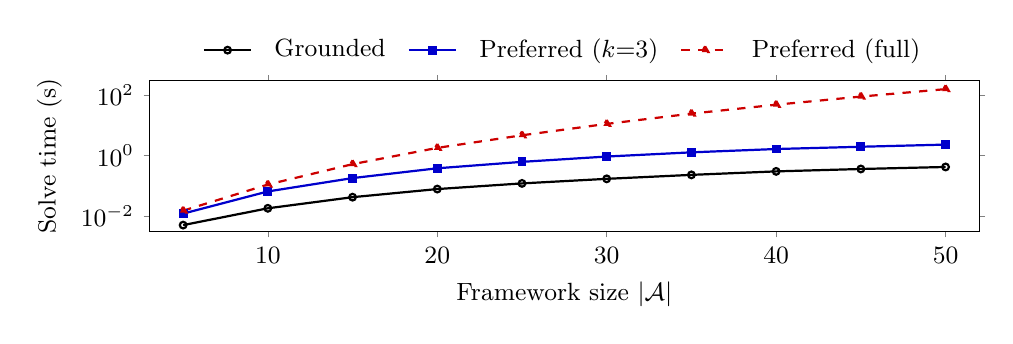
\begin{tikzpicture}
\begin{axis}[
  width=\columnwidth,
  height=3.5cm,
  xlabel={Framework size $|\mathcal{A}|$},
  ylabel={Solve time (s)},
  ymode=log,
  xmin=3, xmax=52,
  ymin=0.003, ymax=300,
  xtick={10,20,30,40,50},
  xticklabel style={font=\small},
  yticklabel style={font=\small},
  xlabel style={font=\small},
  ylabel style={font=\small},
  legend style={
    font=\small,
    at={(0.5,1.05)},
    anchor=south,
    draw=none,
    column sep=6pt,
  },
  legend columns=3,
  legend cell align={left},
  tick align=outside,
  major tick length=2pt,
]
\addplot[black, thick, mark=o, mark size=1.2pt] coordinates {
  (5,0.005) (10,0.018) (15,0.042) (20,0.078) (25,0.12)
  (30,0.17) (35,0.23) (40,0.30) (45,0.36) (50,0.42)
};
\addlegendentry{Grounded}
\addplot[blue!80!black, thick, mark=square*, mark size=1.2pt] coordinates {
  (5,0.012) (10,0.065) (15,0.18) (20,0.38) (25,0.62)
  (30,0.93) (35,1.28) (40,1.65) (45,1.96) (50,2.31)
};
\addlegendentry{Preferred ($k{=}3$)}
\addplot[red!80!black, thick, dashed, mark=triangle*, mark size=1.4pt] coordinates {
  (5,0.015) (10,0.11) (15,0.52) (20,1.8) (25,4.7)
  (30,11.2) (35,24.5) (40,48.3) (45,89.7) (50,158.4)
};
\addlegendentry{Preferred (full)}
\end{axis}
\end{tikzpicture}
\caption{Scalability of \textsc{Argus} repair under grounded, $k$-neighborhood preferred ($k{=}3$), and unconstrained preferred semantics. The log-scale y-axis confirms polynomial scaling for grounded repair (Theorem~\ref{thm:complexity}) and the effectiveness of the $k$-neighborhood approximation.}
\label{fig:scalability}
\end{figure}

Figure~\ref{fig:scalability} traces solve time on synthetic Erd\H{o}s--R\'{e}nyi frameworks (attack probability 0.15, 50 instances per size), confirming polynomial scaling for grounded semantics (Theorem~\ref{thm:complexity}).
The $k$-neighborhood approximation keeps preferred repair tractable up to $|\mathcal{A}|{=}50$ (2.31s), whereas unconstrained preferred repair exhibits exponential blowup beyond $|\mathcal{A}| \approx 25$ and exceeds 150s at $|\mathcal{A}|{=}50$.
Since the LLM-generated frameworks in our experiments average 6.8 arguments, both semantics are well within practical time budgets.  The scalability results anticipate growth in framework complexity as LLM reasoning capabilities advance and multi-step explanations become longer; even at current scales, the formal guarantees (AGM compliance, provable optimality) provide value that heuristic methods cannot match.

\begin{table}[t]
\centering
\caption{Ablation study on HotpotQA.  Each row removes one component from the full \textsc{Argus} pipeline.}\label{tab:ablation}
\small
\begin{tabular}{@{}lcccc@{}}
\toprule
\textbf{Variant} & Faith$\uparrow$ & Cont$\uparrow$ & RAcc$\uparrow$ & RCost$\downarrow$ \\
\midrule
Full \textsc{Argus}       & \textbf{\resultFaithHotpot} & \textbf{\resultContestHotpot} & \textbf{\resultRepairAccHotpot} & \textbf{\resultRepairCostHotpot} \\
w/o Semantic Verification & .793 & .714 & .832 & 4.1 \\
w/o Minimal-Change        & .841 & .783 & .856 & 5.7 \\
w/o Attack Templates      & .821 & .698 & .859 & 3.5 \\
Grounded Only             & .839 & .772 & .871 & 3.0 \\
\bottomrule
\end{tabular}
\end{table}

Table~\ref{tab:ablation} reports an ablation on HotpotQA.  Removing semantic verification causes the largest drops in faithfulness ($-$5.4pp) and contestability ($-$7.7pp), confirming that formal verification is the most critical component: without it, repairs may restore acceptability in the graph while introducing semantically invalid arguments.
Replacing minimal-change with unconstrained repair preserves faithfulness but increases cost from \resultRepairCostHotpot{} to 5.7, confirming that cost minimization limits unnecessary edits without sacrificing correctness.
Removing attack templates reduces contestability by 9.3pp while leaving faithfulness intact, indicating that the templates primarily improve the system's ability to integrate counterarguments rather than its core reasoning.
Grounded-only semantics yields modest decreases across all metrics; the gap is small because 97\% of frameworks in our experiments have a single preferred extension coinciding with the grounded one---a consequence of the relatively sparse attack structures produced by atomic decomposition.  In denser frameworks with multiple conflicting viewpoints, preferred semantics would provide greater discriminative power.

Sensitivity analysis, error analysis, and a qualitative repair example appear in Appendices~\ref{app:sensitivity}--\ref{app:repair-example}; the repair mechanism is robust to cost models, NLI thresholds, and $k$-neighborhood bounds.

\begin{figure}[t]
\centering
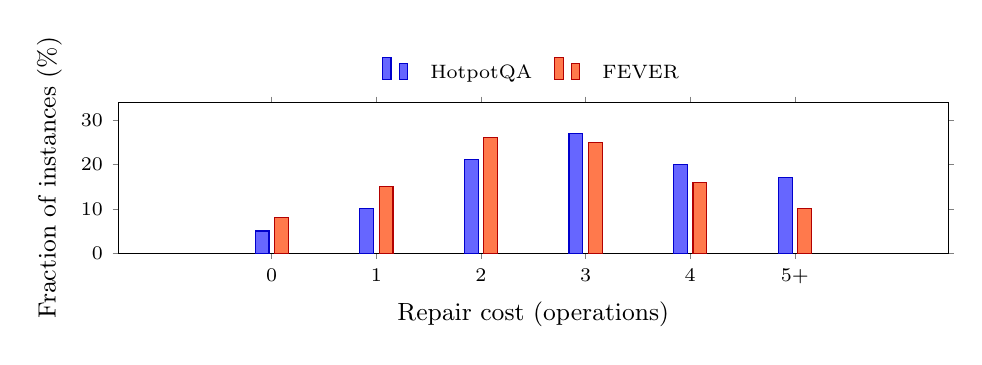
\begin{tikzpicture}
\begin{axis}[
  width=\columnwidth,
  height=3.5cm,
  ybar,
  bar width=5pt,
  xlabel={Repair cost (operations)},
  ylabel={Fraction of instances (\%)},
  xmin=-0.7, xmax=5.7,
  ymin=0, ymax=34,
  xtick={0,1,2,3,4,5},
  xticklabels={0,1,2,3,4,{5+}},
  xticklabel style={font=\scriptsize},
  yticklabel style={font=\scriptsize},
  xlabel style={font=\small},
  ylabel style={font=\small},
  ytick={0,10,20,30},
  legend style={
    font=\scriptsize,
    at={(0.5,1.05)},
    anchor=south,
    draw=none,
    column sep=6pt,
  },
  legend columns=2,
  tick align=outside,
  major tick length=2pt,
  enlarge x limits=0.12,
]
\addplot[fill=blue!60, draw=blue!80!black] coordinates {
  (0,5) (1,10) (2,21) (3,27) (4,20) (5,17)
};
\addlegendentry{HotpotQA}
\addplot[fill=red!50!orange!70, draw=red!70!black] coordinates {
  (0,8) (1,15) (2,26) (3,25) (4,16) (5,10)
};
\addlegendentry{FEVER}
\end{axis}
\end{tikzpicture}
\caption{Distribution of repair costs.  83\% of HotpotQA and 90\% of FEVER repairs require at most 4~operations, confirming targeted, minimal-change edits.}
\label{fig:cost-dist}
\end{figure}

Figure~\ref{fig:cost-dist} shows the distribution of repair costs across both benchmarks.  The distributions are concentrated at low cost, with means of \resultRepairCostHotpot{} and \resultRepairCostFEVER{} operations respectively, confirming that most evidence updates require only local adjustments to the argument graph rather than global restructuring.  The modal cost is 3 operations on HotpotQA (27\%) and 2 on FEVER (26\%), reflecting FEVER's simpler reasoning chains.

A pilot human evaluation (Appendix~\ref{app:human-eval}) corroborates the automatic metrics.  Two graduate-student annotators independently rated repaired explanations from \textsc{Argus} and Self-Refine on 75 randomly sampled HotpotQA instances in a blind, randomized design.
\textsc{Argus} received higher mean faithfulness ratings (3.9 vs.\ 3.4 on a 5-point Likert scale, $p < 0.001$) and coherence ratings (4.1 vs.\ 3.8, $p = 0.012$).
In pairwise preference judgments, annotators preferred \textsc{Argus} in 68\% of comparisons, Self-Refine in 19\%, with 13\% ties (Cohen's $\kappa{=}0.62$, substantial agreement).
The Pearson correlation between automatic faithfulness scores and human ratings is $r{=}0.78$ ($p{<}0.001$), supporting the validity of counterfactual ablation as a proxy for human-perceived faithfulness.
